\documentclass[11pt]{article}

% Increase main memory size
\usepackage{etex}
\usepackage{morewrites}
\usepackage{multicol}
\usepackage{pgfplots}
\usepackage{tikz}
\usetikzlibrary{external}
\tikzexternalize[prefix=cached_models/]
% Ensure the directory exists
\immediate\write18{mkdir -p cached_models}

\usepackage{etex}
\usepackage{morewrites}
\usepackage{enumitem}
\usepackage{float}

\listfiles

\usepackage{amsmath, amssymb, amsthm}
\usepackage{graphicx}
\usepackage{geometry}
\usepackage{array}
\usepackage{booktabs}
\usepackage{float}
\usepackage{verbatim}
\usetikzlibrary{3d}

% Page Layout
\geometry{a4paper, margin=1in}
\setlength\parindent{0pt}
\pgfplotsset{compat=1.18}

% Custom commands
\newcommand{\card}[1]{\lvert #1 \rvert}
\newcommand{\inner}[2]{\left\langle #1, #2 \right\rangle}

\title{\textbf{Principles of Mathematical Analysis}}
\author{}
\date{}

\begin{document}

\maketitle

\section{Measure Theory}
\subsection{Riemann Integral}
For a bounded function \( f: [a, b] \to \mathbb{R} \) and any partition of the interval \([a, b]\), \(P = \{a = x_0 < x_1 < \ldots < x_n = b\}\), we consider on each subinterval \(I_j = [x_{j-1}, x_j], \quad j = 1, \ldots, n\), the quantities:
\[M_j = \sup_{x \in I_j} f(x), \quad m_j = \inf_{x \in I_j} f(x).\]

We also define the upper and lower sums of \(f\) with respect to the partition \(P\) as:
\[U_f(P) = \sum_{j=1}^{n} M_j (x_j - x_{j-1}), \quad L_f(P) = \sum_{j=1}^{n} m_j (x_j - x_{j-1}).\]

\begin{center}
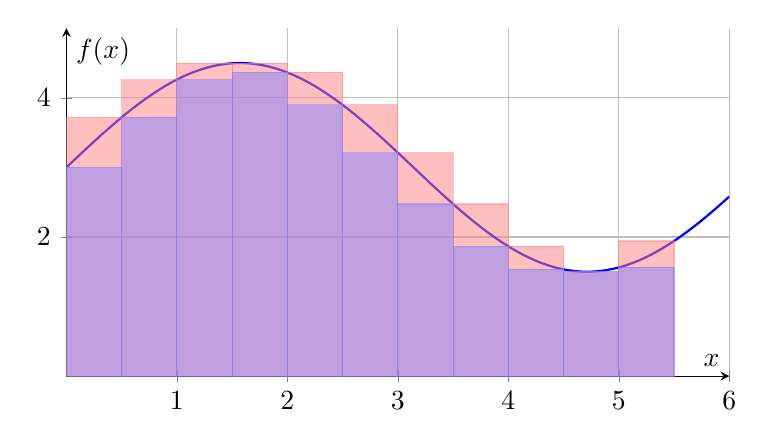
\begin{tikzpicture}
    \begin{axis}[
        axis lines = middle,
        xlabel = \(x\),
        ylabel = {\(f(x)\)},
        domain=0:6,
        samples=100,
        ymin=0, ymax=5,
        xmin=0, xmax=6,
        width=10cm,
        height=6cm,
        grid=both,
    ]
    \addplot[blue, thick] {1.5*sin(deg(x)) + 3};
    \addplot[red!50, fill=red!50, opacity=0.5] coordinates {(0,0) (0,{1.5*sin(deg(0.5))+3}) (0.5,{1.5*sin(deg(0.5))+3}) (0.5,0)} -- cycle;
    \addplot[red!50, fill=red!50, opacity=0.5] coordinates {(0.5,0) (0.5,{1.5*sin(deg(1))+3}) (1,{1.5*sin(deg(1))+3}) (1,0)} -- cycle;
    \addplot[red!50, fill=red!50, opacity=0.5] coordinates {(1,0) (1,{1.5*sin(deg(1.5))+3}) (1.5,{1.5*sin(deg(1.5))+3}) (1.5,0)} -- cycle;
    \addplot[red!50, fill=red!50, opacity=0.5] coordinates {(1.5,0) (1.5,{1.5*sin(deg(1.5))+3}) (2,{1.5*sin(deg(1.5))+3}) (2,0)} -- cycle;
    \addplot[red!50, fill=red!50, opacity=0.5] coordinates {(2,0) (2,{1.5*sin(deg(2))+3}) (2.5,{1.5*sin(deg(2))+3}) (2.5,0)} -- cycle;
    \addplot[red!50, fill=red!50, opacity=0.5] coordinates {(2.5,0) (2.5,{1.5*sin(deg(2.5))+3}) (3,{1.5*sin(deg(2.5))+3}) (3,0)} -- cycle;
    \addplot[red!50, fill=red!50, opacity=0.5] coordinates {(3,0) (3,{1.5*sin(deg(3))+3}) (3.5,{1.5*sin(deg(3))+3}) (3.5,0)} -- cycle;
    \addplot[red!50, fill=red!50, opacity=0.5] coordinates {(3.5,0) (3.5,{1.5*sin(deg(3.5))+3}) (4,{1.5*sin(deg(3.5))+3}) (4,0)} -- cycle;
    \addplot[red!50, fill=red!50, opacity=0.5] coordinates {(4,0) (4,{1.5*sin(deg(4))+3}) (4.5,{1.5*sin(deg(4))+3}) (4.5,0)} -- cycle;
    \addplot[red!50, fill=red!50, opacity=0.5] coordinates {(4.5,0) (4.5,{1.5*sin(deg(4.66))+3}) (5,{1.5*sin(deg(4.66))+3}) (5,0)} -- cycle;
    \addplot[red!50, fill=red!50, opacity=0.5] coordinates {(5,0) (5,{1.5*sin(deg(5.5))+3}) (5.5,{1.5*sin(deg(5.5))+3}) (5.5,0)} -- cycle;

    \addplot[blue!50, fill=blue!50, opacity=0.5] coordinates {(0,0) (0,{1.5*sin(deg(0))+3}) (0.5,{1.5*sin(deg(0))+3}) (0.5,0)} -- cycle;
    \addplot[blue!50, fill=blue!50, opacity=0.5] coordinates {(0.5,0) (0.5,{1.5*sin(deg(0.5))+3}) (1,{1.5*sin(deg(0.5))+3}) (1,0)} -- cycle;
    \addplot[blue!50, fill=blue!50, opacity=0.5] coordinates {(1,0) (1,{1.5*sin(deg(1))+3}) (1.5,{1.5*sin(deg(1))+3}) (1.5,0)} -- cycle;
    \addplot[blue!50, fill=blue!50, opacity=0.5] coordinates {(1.5,0) (1.5,{1.5*sin(deg(2))+3}) (2,{1.5*sin(deg(2))+3}) (2,0)} -- cycle;
    \addplot[blue!50, fill=blue!50, opacity=0.5] coordinates {(2,0) (2,{1.5*sin(deg(2.5))+3}) (2.5,{1.5*sin(deg(2.5))+3}) (2.5,0)} -- cycle;
    \addplot[blue!50, fill=blue!50, opacity=0.5] coordinates {(2.5,0) (2.5,{1.5*sin(deg(3))+3}) (3,{1.5*sin(deg(3))+3}) (3,0)} -- cycle;
    \addplot[blue!50, fill=blue!50, opacity=0.5] coordinates {(3,0) (3,{1.5*sin(deg(3.5))+3}) (3.5,{1.5*sin(deg(3.5))+3}) (3.5,0)} -- cycle;
    \addplot[blue!50, fill=blue!50, opacity=0.5] coordinates {(3.5,0) (3.5,{1.5*sin(deg(4))+3}) (4,{1.5*sin(deg(4))+3}) (4,0)} -- cycle;
    \addplot[blue!50, fill=blue!50, opacity=0.5] coordinates {(4,0) (4,{1.5*sin(deg(4.5))+3}) (4.5,{1.5*sin(deg(4.5))+3}) (4.5,0)} -- cycle;
    \addplot[blue!50, fill=blue!50, opacity=0.5] coordinates {(4.5,0) (4.5,{1.5*sin(deg(4.66))+3}) (5,{1.5*sin(deg(4.66))+3}) (5,0)} -- cycle;
    \addplot[blue!50, fill=blue!50, opacity=0.5] coordinates {(5,0) (5,{1.5*sin(deg(5))+3}) (5.5,{1.5*sin(deg(5))+3}) (5.5,0)} -- cycle;
    \end{axis}
\end{tikzpicture}
\end{center}

For any two partitions \(P\) and \(Q\) of \([a, b]\), we have:
\[L_f(P) \leq \text{Area under } f \leq U_f(Q).\]

If $P$ has a value $I$ such that:
\[\sup_{P} L_f(P) = I = \inf_{P} U_f(P),\]
then we say that \(f\) is Riemann integrable on \([a, b]\) and define the Riemann integral of \(f\) over \([a, b]\) as:
\[\int_a^b f(x) \, dx = I.\]

Continuous functions on closed intervals are Riemann integrable.
\subsection{The Lebesgue Integral}
A bounded function \( f: [a, b] \to \mathbb{R} \) is said to be \textit{Lebesgue integrable} on \([a, b]\) if the set of points where \(f\) is discontinuous has zero measure. 

A set $B \subset \mathbb{R}$ has \textit{measure zero} if for every $\varepsilon > 0$, it can be covered by a countable collection of open intervals $\{(a_n, b_n)\}$ such that:
\[B \subset \bigcup_{n=1}^{\infty} (a_n, b_n) \quad \text{and} \quad \sum_{n=1}^{\infty} (b_n - a_n) < \varepsilon.\]

\subsubsection{Example: Dirichlet Function}
The Dirichlet function:
\[ f(x) = \chi_{\mathbb{Q}}(x) = \begin{cases} 1 & \text{if } x \in \mathbb{Q}, \\ 0 & \text{if } x \notin \mathbb{Q}, \end{cases} \]

On the interval \([0, 1]\): 
\begin{center}
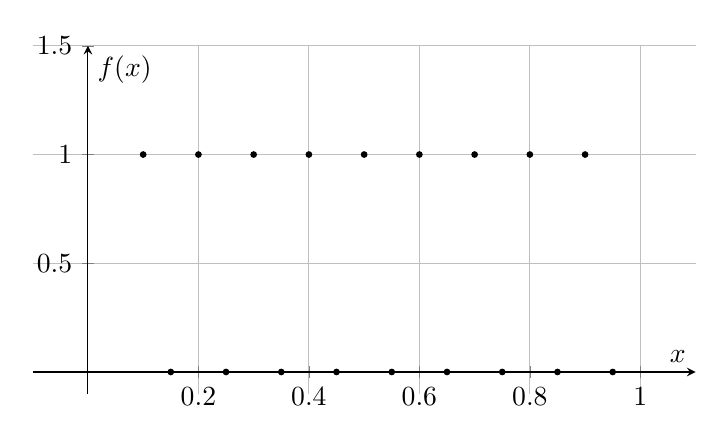
\begin{tikzpicture}
    \begin{axis}[
        axis lines = middle,
        xlabel = \(x\),
        ylabel = {\(f(x)\)},
        domain=0:1,
        samples=100,
        ymin=-0.1, ymax=1.5,
        xmin=-0.1, xmax=1.1,
        width=10cm,
        height=6cm,
        grid=both,
    ]
    \addplot[only marks, mark=*, mark size=1pt] coordinates {
        (0.1,1) (0.2,1) (0.3,1) (0.4,1) (0.5,1) (0.6,1) (0.7,1) (0.8,1) (0.9,1)
        (0.15,0) (0.25,0) (0.35,0) (0.45,0) (0.55,0) (0.65,0) (0.75,0) (0.85,0) (0.95,0)
    };
    \end{axis}
\end{tikzpicture}
\end{center}

We see that \(f\) is not Riemann integrable since it is discontinuous everywhere. 

But consider, 
\[\mathbb{Q} = \{q_1, q_2, q_3, \ldots\}\] 
and define:
\[f_1(x) = \chi_{\{q_1\}}(x) \rightarrow \text{integrable on } [0, 1]\]
\[f_2(x) = \chi_{\{q_1, q_2\}}(x) \rightarrow \text{integrable on } [0, 1]\]
\[\vdots\]
\[f_n(x) = \chi_{\{q_1, q_2, \ldots, q_n\}}(x) \rightarrow \text{integrable on } [0, 1]\]

Then,
\[\lim_{n \to \infty} f_n(x) = \chi_{\mathbb{Q}}(x).\]

\subsubsection{Characteristic Function}
For any set \(A \subset \mathbb{R}\), the characteristic function \(\chi_A: \mathbb{R} \to \{0, 1\}\) is defined as:
\[\chi_A(x) = \begin{cases} 1 & \text{if } x \in A, \\ 0 & \text{if } x \notin A. \end{cases}\]

\[\int_0^1 f_1(x) \, dx = 0 = \int_0^1 f_2(x) \, dx = \ldots = \int_0^1 f_n(x) \, dx = 0.\]

\subsubsection*{Example}
Let 
\[f_n(x) = \begin{cases} x^n & \text{if } 0 \leq x < 1, \\ 0 & \text{if } 1 \leq x. \end{cases}\]

Then, with $f_n(x)$ continuous on $\mathbb{R}$, we have:

\[\lim_{n \to \infty} f_n(x) = \begin{cases} 0 & \text{if } 0 \leq x < 1, \\ 1 & \text{if } x \leq 1. \end{cases}\]

so we can see that there is a discontinuity at \(x = 1\).

\begin{center}
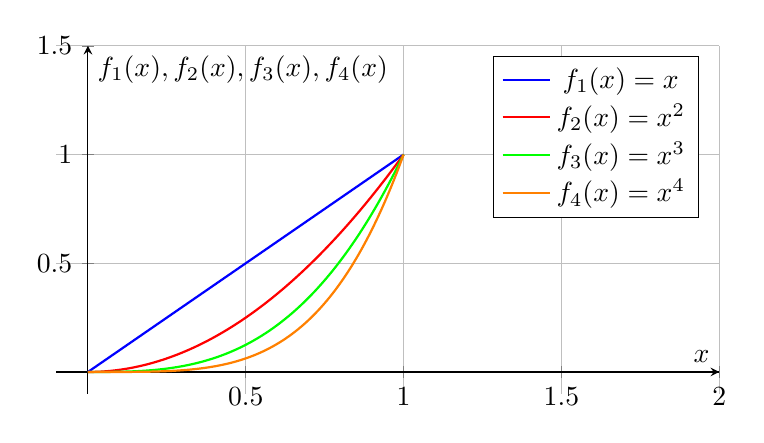
\begin{tikzpicture}
    \begin{axis}[
        axis lines = middle,
        xlabel = \(x\),
        ylabel = {\(f_1(x), f_2(x), f_3(x), f_4(x)\)},
        domain=0:1,
        samples=100,
        ymin=-0.1, ymax=1.5,
        xmin=-0.1, xmax=2,
        width=10cm,
        height=6cm,
        grid=both,
        legend pos=north east
    ]
    \addplot[blue, thick] {x};
    \addlegendentry{\(f_1(x) = x\)}

    \addplot[red, thick] {x^2};
    \addlegendentry{\(f_2(x) = x^2\)}

    \addplot[green, thick] {x^3};
    \addlegendentry{\(f_3(x) = x^3\)}

    \addplot[orange, thick] {x^4};
    \addlegendentry{\(f_4(x) = x^4\)}

    \addplot[black, thick] coordinates {(1,0) (2,0)};
    \end{axis}
\end{tikzpicture}
\end{center}

\subsubsection*{Example}
Let
\[f_n(x) = \begin{cases} -1 & \text{if } x \leq -\frac{1}{n}, \\ \sin\left(\dfrac{n\pi x}{2}\right) & \text{if } -\frac{1}{n} \leq x \leq \frac{1}{n}, \\ 1 & \text{if } \frac{1}{n} \leq x. \end{cases}\]

Then, with $f_n(x)$ continuous and differentiable on $\mathbb{R}$, we have:
\[\lim_{n \to \infty} f_n(x) = \begin{cases} -1 & \text{if } x < 0, \\ 0 & \text{if } x = 0, \\ 1 & \text{if } x > 0. \end{cases}\]
\begin{center}
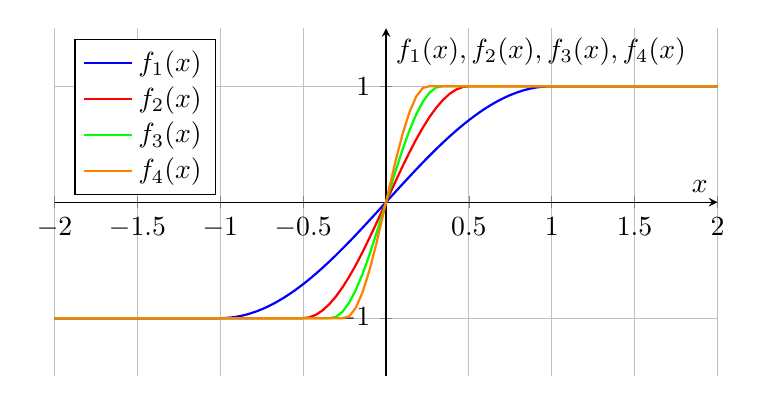
\begin{tikzpicture}
    \begin{axis}[
        axis lines = middle,
        xlabel = \(x\),
        ylabel = {\(f_1(x), f_2(x), f_3(x), f_4(x)\)},
        domain=-2:2,
        samples=100,
        ymin=-1.5, ymax=1.5,
        xmin=-2, xmax=2,
        width=10cm,
        height=6cm,
        grid=both,
        legend pos=north west
    ]
    \addplot[blue, thick] {x <= -1 ? -1 : (x >= 1 ? 1 : sin(deg(pi*x/2)))};
    \addlegendentry{\(f_1(x)\)}

    \addplot[red, thick] {x <= -0.5 ? -1 : (x >= 0.5 ? 1 : sin(deg(2*pi*x/2)))};
    \addlegendentry{\(f_2(x)\)}

    \addplot[green, thick] {x <= -0.33 ? -1 : (x >= 0.33 ? 1 : sin(deg(3*pi*x/2)))};
    \addlegendentry{\(f_3(x)\)}

    \addplot[orange, thick] {x <= -0.25 ? -1 : (x >= 0.25 ? 1 : sin(deg(4*pi*x/2)))};
    \addlegendentry{\(f_4(x)\)}
    \end{axis}
\end{tikzpicture}
\end{center}

\subsubsection*{Example}
The Dirichlet function is not integrable but it is the limit of a sequence of integrable functions, all with integral equal to zero.

We need to define a new kind of convergence.

\subsection{Convergences}
A sequence of functions \(\{f_n\}_{n \in \mathbb{N}}\) converges punctually to a function \(f\) on \(Dom(f)\) if:
\[\lim_{n \to \infty} f_n(x) = f(x), \quad \forall x \in Dom(f).\]

\[\forall \varepsilon > 0, \quad \forall x \in Dom(f), \quad \exists N (\varepsilon, x) \in \mathbb{N} : n > N \implies |f_n(x) - f(x)| < \varepsilon.\]

A sequence of functions \(\{f_n\}_{n \in \mathbb{N}}\) converges uniformly to a function \(f\) on \(Dom(f)\) if:
\[\forall \varepsilon, \quad \exists N : n > N \implies |f_n(x) - f(x)| < \varepsilon, \quad \forall x \in Dom(f).\]

\subsubsection*{Example}
Let
\[f_n(x) = \frac{1}{n} \sin(nx), \quad x \in \mathbb{R}. \rightarrow^{n\to\infty} f(x) = 0.\]

\begin{center}
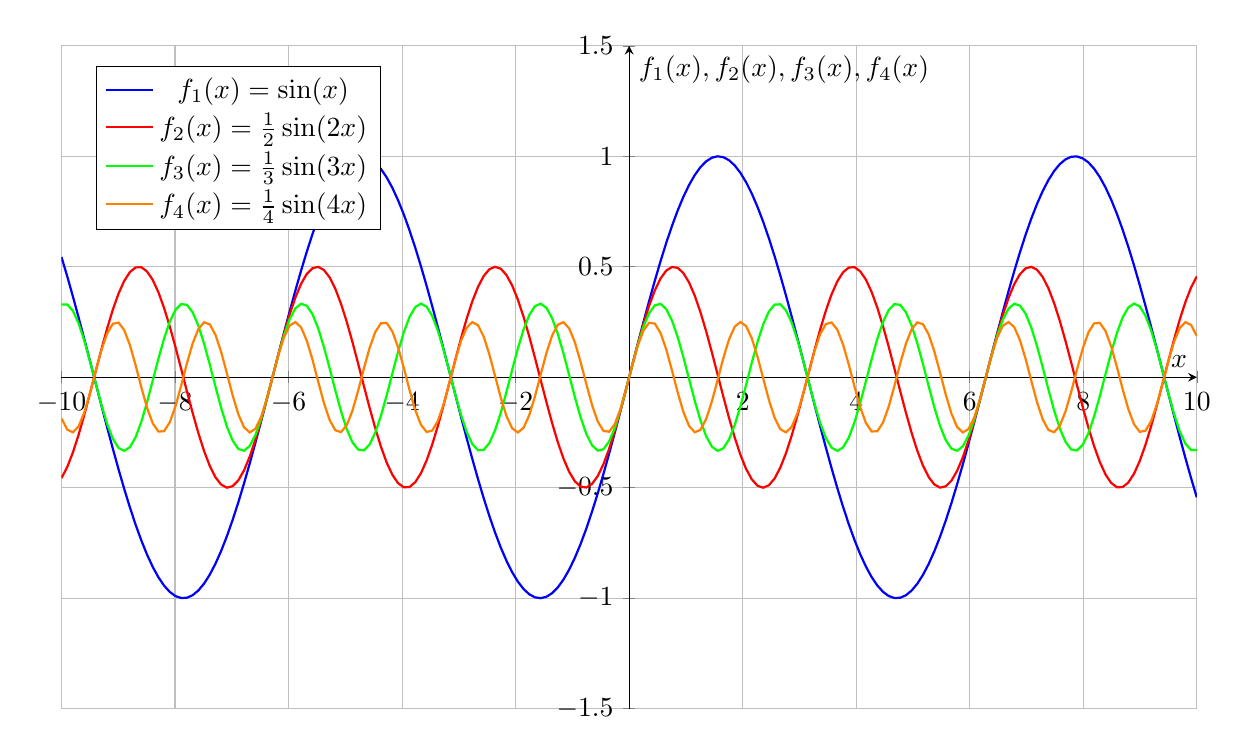
\begin{tikzpicture}
    \begin{axis}[
        axis lines = middle,
        xlabel = \(x\),
        ylabel = {\(f_1(x), f_2(x), f_3(x), f_4(x)\)},
        domain=-10:10,
        samples=200,
        ymin=-1.5, ymax=1.5,
        xmin=-10, xmax=10,
        width=16cm,
        height=10cm,
        grid=both,
        legend pos=north west
    ]
    \addplot[blue, thick] {1*sin(deg(x))};
    \addlegendentry{\(f_1(x) = \sin(x)\)}

    \addplot[red, thick] {1/2*sin(deg(2*x))};
    \addlegendentry{\(f_2(x) = \frac{1}{2}\sin(2x)\)}

    \addplot[green, thick] {1/3*sin(deg(3*x))};
    \addlegendentry{\(f_3(x) = \frac{1}{3}\sin(3x)\)}

    \addplot[orange, thick] {1/4*sin(deg(4*x))};
    \addlegendentry{\(f_4(x) = \frac{1}{4}\sin(4x)\)}
    \end{axis}
\end{tikzpicture}
\end{center}

\subsubsection{Uniform Convergence}
\begin{enumerate}
    \item If \(\{f_n\}_{n \in \mathbb{N}}\) converges uniformly to \(f\) on \([a, b]\) and each \(f_n\) is continuous, then:
        \[\int_a^b f(x) \, dx = \lim_{n \to \infty} \int_a^b f_n(x) \, dx.\]
    \item If \(\{f_n\}_{n \in \mathbb{N}}\) converges uniformly to \(f\) on \([a, b]\) and each \(f_n\) is continuous in \([a, b]\), then \(f\) is continuous on \([a, b]\).
    \item If \(\{f_n\}_{n \in \mathbb{N}}\) is a sequence of differentiable functions on \([a, b]\) that converges punctually to some continuous function \(f\) on \([a, b]\) and if the sequence of derivatives \(\{f_n'\}_{n \in \mathbb{N}}\) converges uniformly to some continuous function \(g\), then \(f\) is differentiable on \((a, b)\) and:
        \[f'(x) = g(x) = \lim_{n \to \infty} f_n'(x).\]
\end{enumerate}

\subsubsection{Henri Lebesgue (1875-1941)}
How can we count money in bills?
\begin{enumerate}
    \item Add each amount as the bills come in. (Riemann)
    \item Make groups by denomination and count each group. (Lebesgue)
\end{enumerate}

This is the idea behind the Lebesgue integral.

\subsection{Cantor Ternary Set}
\vskip 1em
\begin{center}
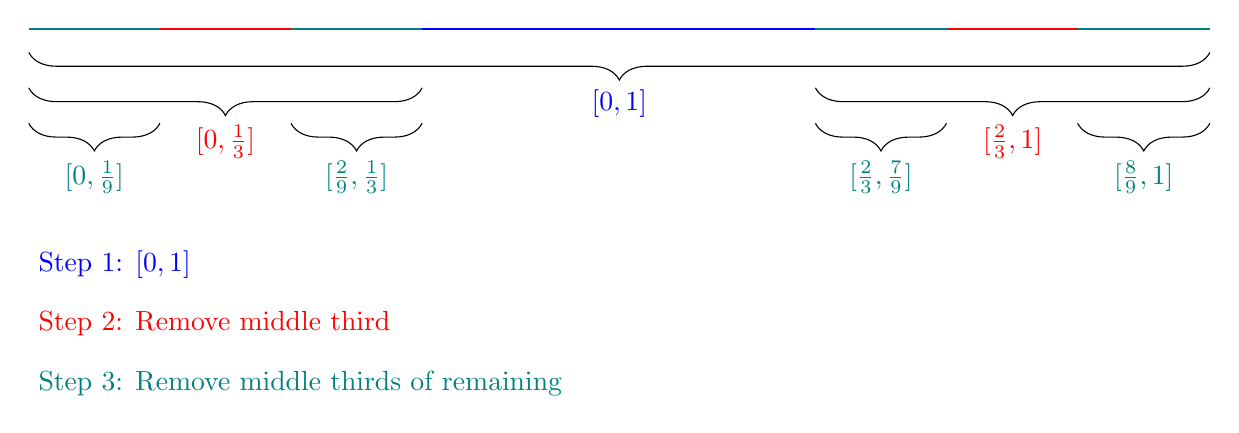
\begin{tikzpicture}[scale=1.5]
    % Step 1
    \draw[thick, blue] (0, 0) -- (10, 0);
    \draw[decorate, decoration={brace, mirror, amplitude=10pt}] (0, -0.2) -- (10, -0.2) node[midway, below=10pt] {\textcolor{blue}{\([0, 1]\)}};

    % Step 2
    \draw[thick, red] (0, 0) -- (3.33, 0);
    \draw[thick, red] (6.66, 0) -- (10, 0);
    \draw[decorate, decoration={brace, mirror, amplitude=10pt}] (0, -0.5) -- (3.33, -0.5) node[midway, below=10pt] {\textcolor{red}{\([0, \frac{1}{3}]\)}};
    \draw[decorate, decoration={brace, mirror, amplitude=10pt}] (6.66, -0.5) -- (10, -0.5) node[midway, below=10pt] {\textcolor{red}{\([\frac{2}{3}, 1]\)}};

    % Step 3
    \draw[thick, teal] (0, 0) -- (1.11, 0);
    \draw[thick, teal] (2.22, 0) -- (3.33, 0);
    \draw[thick, teal] (6.66, 0) -- (7.77, 0);
    \draw[thick, teal] (8.88, 0) -- (10, 0);
    \draw[decorate, decoration={brace, mirror, amplitude=10pt}] (0, -0.8) -- (1.11, -0.8) node[midway, below=10pt] {\textcolor{teal}{\([0, \frac{1}{9}]\)}};
    \draw[decorate, decoration={brace, mirror, amplitude=10pt}] (2.22, -0.8) -- (3.33, -0.8) node[midway, below=10pt] {\textcolor{teal}{\([\frac{2}{9}, \frac{1}{3}]\)}};
    \draw[decorate, decoration={brace, mirror, amplitude=10pt}] (6.66, -0.8) -- (7.77, -0.8) node[midway, below=10pt] {\textcolor{teal}{\([\frac{2}{3}, \frac{7}{9}]\)}};
    \draw[decorate, decoration={brace, mirror, amplitude=10pt}] (8.88, -0.8) -- (10, -0.8) node[midway, below=10pt] {\textcolor{teal}{\([\frac{8}{9}, 1]\)}};

    % Legend
    \node[anchor=west] at (0, -2) {\textcolor{blue}{Step 1: \([0, 1]\)}};
    \node[anchor=west] at (0, -2.5) {\textcolor{red}{Step 2: Remove middle third}};
    \node[anchor=west] at (0, -3) {\textcolor{teal}{Step 3: Remove middle thirds of remaining}};
\end{tikzpicture}
\end{center}

The Cantor set \(C\) is obtained by removing the open middle third of each remaining interval at each step. Then,
\[C = [0, 1] \setminus J = \bigcup_{n=1}^{\infty} J_n,\]
where \(J\) is the union of all removed intervals and \(J_n\) is the set remaining after \(n\) steps. For the measure of \(C\):
\[\card{J} = \sum_{n=1}^{\infty} \card{J_n} = \sum_{n=1}^{\infty} \frac{2^{n-1}}{3^n} = \frac{1}{3} + \frac{2}{9} + \frac{4}{27} + \ldots = 1.\]
Thus, the measure of the Cantor set \(C\) is:
\[\card{C} = \card{[0, 1]} - \card{J} = 1 - 1 = 0.\]

The Cantor set is not empty; it contains points such as 0, 1, and all endpoints of the removed intervals. It has the following properties:
\begin{itemize}
    \item It does not contain any intervals.
    \item It is closed and bounded, hence compact.
    \item It is a perfect set, which means it is closed and every point is an accumulation point.
    \item It is uncountable, because there is a bijection between the Cantor set and the interval \([0, 1]\) using ternary representation:
        \[\Phi: [0, 1] \to C,\]
    where each \(x \in C\) is expressed in base 3, and has the form:
        \[x = \sum_{n=1}^{\infty} \frac{a_n}{3^n}, \quad a_n \in \{0, 2\}.\]
        Then, for each \(x \in [0, 1]\) we define:
        \[x = \sum_{n=1}^{\infty} \frac{b_n}{2^n}, \quad b_n \in \{0, 1\}.\]
        We can then define:
        \[\Phi(x) = \sum_{n=1}^{\infty} \frac{2b_n}{3^n}.\]
        Now, \(2b_n \in \{0, 2\}\) so \(\Phi(x) \in C\). This function is bijective, hence \(C\) is uncountable.
\end{itemize}

\section{Measurable Spaces and Topological Spaces}
A \textit{Topological Space} $(X, \mathcal{T})$ is a collection $\cal{T}$ of subsets of a set $X$ in a topology such that:

\begin{itemize}
    \item The empty set $\emptyset$ and the whole set $X$ are in $\mathcal{T}$.
    \item The union of any collection of sets in $\mathcal{T}$ is also in $\mathcal{T}$.
    \item The intersection of any finite number of sets in $\mathcal{T}$ is also in $\mathcal{T}$.
\end{itemize}

\subsubsection*{Example: The Real Line}
Let $X = \mathbb{R}$ and $\mathcal{T}$ be the collection of all open intervals $(a, b)$ where $a < b$ and $a, b \in \mathbb{R}$. Then $(\mathbb{R}, \mathcal{T})$ is a topological space.
One can observe that if, for instance, we take the intersection of open intervals like:
\[\bigcap_{n=1}^{\infty} \left(-\frac{1}{n}, \frac{1}{n}\right) = \{0\},\]
which is not an open set, hence the requirement for finite intersections.
\vskip 1em
The sets in a topology $\mathcal{T}$ are called \textit{open sets}. For example, with $X = \bar{\mathbb{R}} = [-\infty, \infty]$, the open sets are all intervals of the form $(a, b)$ where $a < b$. Then, we say that $(\bar{\mathbb{R}}, \mathcal{T})$ is a topological space.

\subsection{Metric Spaces}
A set $X$ is a \textit{metric space} if there exists a distance function $d: X \times X \to [0, \infty)$, such that for all $x, y, z \in X$:
\begin{itemize}
    \item $d(x, y) = 0$ if and only if $x = y$ (identity of indiscernibles).
    \item $d(x, y) = d(y, x)$ (symmetry).
    \item $d(x, z) \leq d(x, y) + d(y, z)$ (triangle inequality).
\end{itemize}

An open ball of center $x \in X$ and radius $r > 0$ is defined as:
\[B(x, r) = \{y \in X : d(x, y) < r\}.\]

\subsection{Continuity}
A function $f: [a, b] \subset \mathbb{R} \to \mathbb{R}$ is continuous at a point $x_0 \in [a, b]$ if for every $\varepsilon > 0$, there exists a $\delta > 0$ such that for all $x \in [a, b]$:
\[|x - x_0| < \delta \implies |f(x) - f(x_0)| < \varepsilon.\]

\begin{center}
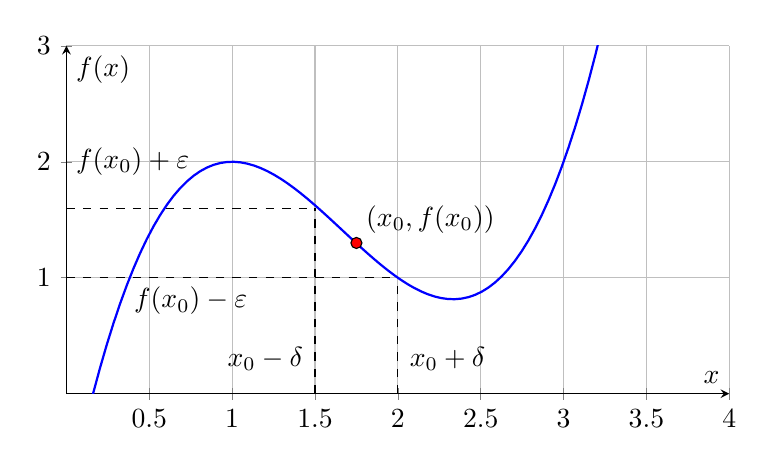
\begin{tikzpicture}
    \begin{axis}[
        axis lines = middle,
        xlabel = \(x\),
        ylabel = {\(f(x)\)},
        domain=0:4,
        samples=100,
        ymin=0, ymax=3,
        xmin=0, xmax=4,
        width=10cm,
        height=6cm,
        grid=both,
    ]
    \addplot[blue, thick] {(x-1)^3 -2*(x-1)^2+ 2};
    \draw[dashed] (1.5,0) -- (1.5,1.6);
    \draw[dashed] (2,0) -- (2,1);
    \draw[dashed] (0,1) -- (2,1);
    \draw[dashed] (0,1.6) -- (1.5,1.6);
    \draw[fill=red] (1.75,1.3) circle (2pt) node[anchor=south west] {\( (x_0, f(x_0)) \)};
    \node at (0.75, 0.8) {\(f(x_0) - \varepsilon\)};
    \node at (0.4, 2) {\(f(x_0) + \varepsilon\)};
    \node at (1.2, 0.3) {\(x_0 - \delta\)};
    \node at (2.3, 0.3) {\(x_0 + \delta\)};
    \end{axis}
\end{tikzpicture}
\end{center}

\subsubsection{Neighborhoods}
A \textit{neighborhood} of a set $A$ is any open set that contains $A$. If $(X, \mathcal{T}_X)$ and $(Y, \mathcal{T}_Y)$ are topological spaces, and $f: X \to Y$ is a mapping, then $f$ is continuous at a point $x_0 \in X$ if for every neighborhood $V$ of $f(x_0)$ in $Y$, there exists a neighborhood $U$ of $x_0$ in $X$ such that:
\[f(U) \subset V.\]

\subsubsection*{Observation}
This is equivalent to the $\varepsilon$-$\delta$ definition on the $\mathbb{R}^n$ spaces.

\subsubsection{Global Continuity}
If $(X, \mathcal{T}_X)$ and $(Y, \mathcal{T}_Y)$ are topological spaces and $f: X \to Y$ is a mapping, then $f$ is globally continuous if:
\[f^{-1}(V) = \{x \in X : f(x) \in V\} \in \mathcal{T}_X, \quad \forall V \in \mathcal{T}_Y.\]
where $f^{-1}(V)$ is the preimage of $V$ under $f$.

\begin{center}
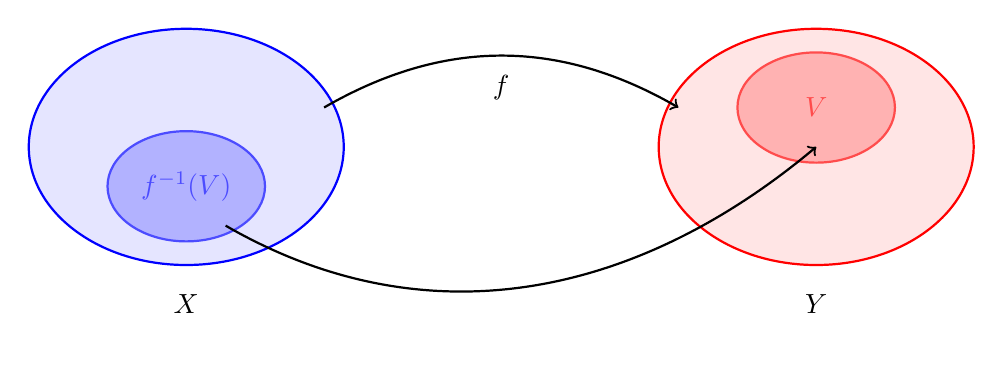
\begin{tikzpicture}
    % Draw blobs for X and Y
    \draw[thick, blue, fill=blue!10] (-2, -1.5) ellipse (2 and 1.5) node {};
    \node at (-2, -3.5) {\(X\)};
    \draw[thick, red, fill=red!10] (6, -1.5) ellipse (2 and 1.5) node {};
    \node at (6, -3.5) {\(Y\)};

    % Sub-blobs for T_X and T_Y
    \draw[thick, blue!70, fill=blue!30] (-2, -2) ellipse (1 and 0.7) node {\(f^{-1}(V)\)};
    \draw[thick, red!70, fill=red!30] (6, -1) ellipse (1 and 0.7) node {\(V\)};

    % Arrows between X and Y
    \draw[->, thick, in=150, out=30] (-0.25, -1) to (4.25, -1);
    \draw[->, thick, in=220, out=330] (-1.5, -2.5) to (6, -1.5);
    \node at (2, -0.75) {\(f\)};
    \node at (2, -3) {\(\)};
\end{tikzpicture}
\end{center}

So, $f$ is continuous if the preimage of every open set in $Y$ is an open set in $X$.

\subsubsection{Proposition}
If $(X, \mathcal{T}_X)$ and $(Y, \mathcal{T}_Y)$ are topological spaces and $f: X \to Y$ is a mapping, then $f$ is continuous if it is continuous at every point $x \in X$.

\subsection{Measurable Spaces}
A collection $\mathcal{A}$ of subsets of a space $X$ is a \textit{$\sigma$-algebra} if:
\begin{enumerate}
    \item $\emptyset \in \mathcal{A}$.
    \item If $A \in \mathcal{A}$, then $A^C\in \mathcal{A}$.
    \item If $\{A_j\}_{j \in \mathbb{N}}$ is a countable collection with each $A_j \in \mathcal{A}$, then:
    \[\bigcup_{j=1}^{\infty} A_j \in \mathcal{A}\]
\end{enumerate}

The sets of $\mathcal{A}$ are called \textit{measurable sets}. The pair $(X, \mathcal{A})$ is called a \textit{measurable space}. If the third property holds for finite collections, then $\mathcal{A}$ is called an \textit{algebra}.

\subsubsection*{Example}
Is $\mathbb{R}$ with the topology of the usual open sets a $\sigma$-algebra?
No, because
\[(a, b) \in \mathcal{T} \text{ but } (a, b)^C = (-\infty, a] \cup [b, \infty) \notin \mathcal{T}.\]

\subsubsection*{Example}
The collection $\mathcal{P}(X)$, the power set of $X$, is a $\sigma$-algebra on $X$.

On $X$, the collection $\{\emptyset, X\}$ is the smallest $\sigma$-algebra.

\subsubsection{Properties of measurable spaces}
If $(X, \mathcal{A})$ is a measurable space, then:
\begin{enumerate}
    \item If $\emptyset \in \mathcal{A}$, then $\emptyset ^C = X \in \mathcal{A}$.
    \item If $A_1, A_2, \ldots, A_n \in \mathcal{A}$, then:
    \[\bigcup_{j=1}^{n} A_j \in \mathcal{A}.\]
    \item If $\{A_j\}_{j \in \mathbb{N}}$ is a countable collection with each $A_j \in \mathcal{A}$ then, following the second property of $\sigma$-algebras:
    \[A_j^C \in \mathcal{A}, \quad \forall j \in \mathbb{N}.\]
    Then, by the third property of $\sigma$-algebras:
    \[\bigcup_{j=1}^{\infty} A_j^C \in \mathcal{A}.\]
    Finally, by the second property again:
    \[\left(\bigcup_{j=1}^{\infty} A_j^C\right)^C = \bigcap_{j=1}^{\infty} A_j \in \mathcal{A}.\]
    \item If $A, B \in \mathcal{A}$, then:
    \[A \setminus B = A \cap B^C \in \mathcal{A}.\]
\end{enumerate}

\subsubsection{Proposition}
If $S \subset \mathcal{P}(X)$, then $\sigma(S)$ is called the $\sigma$-algebra generated by $S$:
\[\sigma(S) = \mathcal{A}_S = \bigcap \{\mathcal{A} : \mathcal{A} \text{ is a } \sigma\text{-algebra and } S \subseteq \mathcal{A} \subseteq \mathcal{P}(X)\}.\]

\subsubsection*{Example}
Let $X = \{1, 2, 3, 4\}$ and $S = \{\{1\}, \{3, 4\}\}$. Then:
\[\sigma(S) = \{\emptyset, X, \{1\}, \{2, 3, 4\}, \{3, 4\}, \{1, 2\}, \{2\}, \{1, 3, 4\}\}.\]

\subsubsection{Borel $\sigma$-algebra}
The Borel $\sigma$-algebra on $X$, denoted by $\mathcal{B}(X)$, is the $\sigma$-algebra generated by the open sets of $X$, 
\[\mathcal{B}(X) = \sigma(\mathcal{T}(X)).\]
Its elements are called \textit{Borel sets}.

\subsubsection*{Example}
The Borel $\sigma$-algebra on $\mathbb{R}$, $\mathcal{B}(\mathbb{R})$, contains all open intervals, closed intervals, countable sets, and complements of these sets. Examples of these Borel sets include:
\[(a, b), \quad [a, b], \quad (a, b], \quad [a, b), \quad \mathbb{Q}, \quad \mathbb{R} \setminus \mathbb{Q}, \quad \{x\}, \quad \mathbb{R}, \quad \emptyset.\]


\end{document}